% $Header: /cvsroot/latex-beamer/latex-beamer/solutions/conference-talks/conference-ornate-20min.en.tex,v 1.7 2007/01/28 20:48:23 tantau Exp $

\documentclass[11pt]{beamer}

\mode<beamer>
{
  \usetheme{default}
  \usecolortheme[rgb={0,0,0.8}]{structure}
  %\setbeamercolor{normal text}{bg=blue!50}
  %\setbeamercolor{normal text}{fg=blue!50}
  % or ...

  %\setbeamercovered{transparent}
  % or whatever (possibly just delete it)
}


\usepackage[english]{babel}
% or whatever

\usepackage[latin1]{inputenc}
% or whatever

\usepackage{times}
\usepackage[T1]{fontenc}
% Or whatever. Note that the encoding and the font should match. If T1
% does not look nice, try deleting the line with the fontenc.

%\usepackage{newcent}
%\usefonttheme{structuresmallcapsserif}

\usepackage{amssymb,latexsym,amsmath}
\usepackage{amsthm}
\DeclareMathOperator*{\argmin}{arg\,min}
\DeclareMathOperator*{\argmax}{arg\,max}

\usepackage{mathtools}
\input xy 
\xyoption{all}
\usepackage[latin1]{inputenc}
\usepackage{color}
\usepackage{tikz}


\title[On Laplacian Eigenmaps for Dimensionality Reduction] % (optional, use only with long paper titles)
{On Laplacian Eigenmaps for Dimensionality Reduction}

%\subtitle

\author[Dr. Juan Orduz] % (optional, use only with lots of authors)
{Dr. Juan Orduz}
% - Give the names in the same order as the appear in the paper.
% - Use the \inst{?} command only if the authors have different
%   affiliation.

\institute[PyData Berlin 2018] % (optional, but mostly needed)
{

}
% - Use the \inst command only if there are several affiliations.
% - Keep it simple, no one is interested in your street address.

\date[ PyData Berlin 2018] % (optional, should be abbreviation of conference name)
{ PyData Berlin 2018}
% - Either use conference name or its abbreviation.
% - Not really informative to the audience, more for people (including
%   yourself) who are reading the slides online

\subject{data science}
% This is only inserted into the PDF information catalog. Can be left
% out.



% If you have a file called "university-logo-filename.xxx", where xxx
% is a graphic format that can be processed by latex or pdflatex,
% resp., then you can add a logo as follows:

\pgfdeclareimage[height=0.7cm]{university-logo}{logo.jpg}
\logo{\pgfuseimage{university-logo}}

% If you wish to uncover everything in a step-wise fashion, uncomment
% the following command:

%\beamerdefaultoverlayspecification{<+->}


\begin{document}

\begin{frame}
  \titlepage
\end{frame}

%\begin{frame}{Contenido}
%\tableofcontents
%\end{frame}

\begin{frame}{Overview}
\tableofcontents
\end{frame}

\section{Introduction}

\begin{frame}{Can One Hear the Shape of a Drum?}{\cite{K66}}
A  {\bf differentiable manifold} is a type of manifold that is locally similar enough to a linear space to allow one to do calculus. A (Riemannian) metric $g$ allow us to measure distances. 
\begin{figure}[h]
\begin{center}
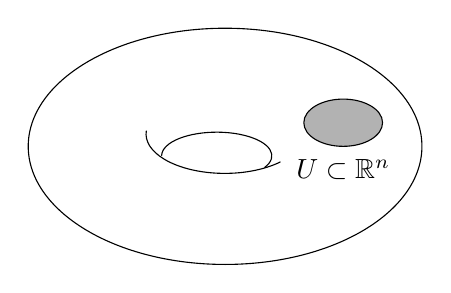
\begin{tikzpicture}
\draw (0,0) ellipse (2.5cm and 1.5cm);
%\draw (-0.5,0) arc (175:315:0.5cm and 0.25cm);
%\draw (0.2,-0.2) arc (-30:180:0.35cm and 0.15cm);
\draw (-1,0.2) arc (175:315:1cm and 0.5cm);
\draw (0.5,-0.27) arc (-30:180:0.7cm and 0.3cm);
\draw [black,fill=gray!60] (1.5,0.3) ellipse (0.5cm and 0.3cm);
\node (a) at (1.5,-0.3) {$U\subset \mathbb{R}^n$};
\end{tikzpicture}
%\caption{$2$-Torus $T^2 = S^1\times S^1$. }
\end{center}
\end{figure}
\pause
We can consider the \textbf{Laplacian} $L:C^\infty(M)\longrightarrow C^\infty(M)$ and its \textbf{spectrum} 
$\text{spec}(L)=\{\lambda_0, \lambda_1, \cdots, \lambda_k, \cdots \longrightarrow \infty\}$. 
\begin{itemize}
\pause
\item If we are given $\text{spec}(L)$ we can infer the dimension of $M$, its volume and its total scalar curvature. 
\end{itemize}
\end{frame}

\begin{frame}{Spectral Geometry for Dimensionality Reduction?}
Let us assume we have data points $x_1, \cdots, x_k\in\mathbb{R}^N$ which lie on an \underline{unknown} submanifold $M\subset\mathbb{R}^N$. 
\begin{block}{Key Observation}
\begin{itemize}
\item Eigenfunctions  of $L$ on $M$ can be used to define lower dimensional embeddings.
\end{itemize}
\end{block}

\begin{block}{Idea (\cite{BN2003})}
\begin{itemize}
\item Model $M$ by constructing a graph $G=(V,E)$ where close data points are connected by edges. 
\pause
\item 
Construct the graph Laplacian $L$ on $G$. 
\pause
\item 
Compute \text{spec}(L) and the corresponding eigenfunctions. 
\pause 
\item Use these eigenfunctions to construct an embedding $F:V\longrightarrow \mathbb{R}^m$ for $m<N$. 
\end{itemize}
\end{block}
\end{frame}

\section{Warming Up}

\subsection{The Spectral Theorem}

\begin{frame}{The Spectral Theorem}
Let $A\in M_{n\times n}(\mathbb{R})$ be a symmetric matrix, i.e. $A=A^\dagger$. 
\pause
\begin{block}{Recall}
\begin{itemize}
\item $\lambda\in\mathbb{C}$ is an {\bf eigenvalue} for A with {\bf eigenvector} $f\in\mathbb{R}^n$, $f\neq 0$, if 
$$Af=\lambda f.$$
\item A set of vectors $\mathcal{B} = \{f_1, f_2, \cdots, f_n\}$ is a {\bf basis} for $\mathbb{R}^n$ if:
\begin{itemize}
\item They are linearly independent. 
\item They generate $\mathbb{R}^n$.
\end{itemize}
\item $\mathcal{B}$ is said to be an {\bf orthonormal} basis if $\langle f_i, f_j\rangle = \delta_{ij}$. 
\end{itemize}
\pause 
\end{block}
\begin{block}{Spectral Theorem}
There exists an orthonormal basis of $\mathbb{R}^n$ consisting of eigenvectors of $A$. Each eigenvalue is real.
\end{block}
\end{frame}

\begin{frame}{Min(Max)imizing Properties of Eigenvalues}
Let $A\in M_n(\mathbb{R})$ be a symmetric matrix with spectral decomposition $\lambda_0 \leq \lambda_1 \leq \cdots \leq \lambda_n$. \\
\vspace{0.3 cm}
For later purposes, we would like to find 
\begin{align*}
\argmax_{||f||=1} \langle Af, f \rangle.
\end{align*}
\begin{itemize}
\pause
\item Define the associated Lagrange optimization problem
\begin{align*}
\mathcal{L}(f, \lambda) = \langle Af, f \rangle -\lambda(||f||^2 - 1).
\end{align*}
\pause
\item Take the derivative with respect to $f$
\begin{align*}
\frac{\partial}{\partial f} \mathcal{L}(f, \lambda) = 2(Af - \lambda f )\stackrel{!}{=} 0.
\end{align*}
\pause
\item Hence, 
\begin{align*}
\argmax_{||f||=1} \langle Af, f \rangle = f_n
\quad \text{and}\quad
\argmin_{||f||=1} \langle Af, f \rangle = f_0.
\end{align*}
\end{itemize}
\end{frame}

\section{Motivation}

\subsection{Toy Model Example}

\begin{frame}{Step 0: Understand the Problem}
Consider the problem of mapping these points to a line so that close points stay as together as possible. 
\begin{figure}[h]
\begin{center}
\begin{tikzpicture}
\node [draw, circle] (a) at (0,0) {1};
\node [draw, circle] (b) at (-0.5,2) {2};
\node [draw, circle] (c) at (0,-1.5) {3};
\node [draw, circle] (d) at (3,0) {4};
\end{tikzpicture}
%\caption{$2$-Torus $T^2 = S^1\times S^1$. }
\end{center}
\end{figure}
\end{frame}

\begin{frame}{Step 1: From Data to Adjacency Graph}
\begin{itemize}
\item Define a distance function: first nearest neighbour.
 \pause
\item For each node, attach an edge for close points. 
\end{itemize}
\begin{figure}[h]
\begin{center}
\begin{tikzpicture}
\node [draw, circle] (a) at (0,0) {1};
\node [draw, circle] (b) at (-0.5,2) {2};
\node [draw, circle] (c) at (0,-1.5) {3};
\node [draw, circle] (d) at (3,0) {4};
\pause
\path [-] (a) edge node[left] {} (c);
\pause
\path [-] (b) edge node[left] {} (a);
\pause
\path [-] (d) edge node[left] {} (a);
\end{tikzpicture}
%\caption{$2$-Torus $T^2 = S^1\times S^1$. }
\end{center}
\end{figure}
\end{frame}

\begin{frame}{Step 2: Construct the Adjacency and Degree Matrices}
\begin{figure}[h]
\begin{center}
\begin{tikzpicture}
\node [draw, circle] (a) at (0,0) {1};
\node [draw, circle] (b) at (-0.5,2) {2};
\node [draw, circle] (c) at (0,-1.5) {3};
\node [draw, circle] (d) at (3,0) {4};
\path [-] (a) edge node[left] {} (c);
\path [-] (b) edge node[left] {} (a);
\path [-] (d) edge node[left] {} (a);
\end{tikzpicture}
%\caption{$2$-Torus $T^2 = S^1\times S^1$. }
\end{center}
\end{figure}
\begin{align*}
W = \left(
\begin{array}{cccc}
 0 & 1 & 1 & 1 \\
 1 & 0 & 0 & 0 \\
 1 & 0 & 0 & 0 \\
 1 & 0 & 0 & 0 
\end{array}
\right)
\quad 
D = \left(
\begin{array}{cccc}
 3 & 0 & 0 & 0 \\
 0 & 1 & 0 & 0 \\
 0 & 0 & 1 & 0 \\
 0 & 0 & 0 & 1 
\end{array}
\right)
\end{align*}
\end{frame}

\begin{frame}{Step 3: Spectrum of the Graph Laplacian}
\begin{itemize}
\item Construct the operator $L$ defined by

\begin{align*}
L \coloneqq D - W  = \left(
\begin{array}{cccc}
 3 & -1 & -1 & -1 \\
 -1 & 1 & 0 & 0 \\
 -1 & 0 & 1 & 0 \\
 -1 & 0 & 0 & 1 
\end{array}
\right)
\end{align*}

\item Consider the generalized eigenvalue problem 
$$Lf = \lambda D f.$$
Equivalently, $D^{-1}Lf = \lambda f$. 
\pause
\item Eigenvalues: $\lambda_0 =0 , \lambda_1 =1, \lambda_2 = 1, \lambda_3 =2$.
\pause
\item An eigenvector for $\lambda_1 = 1$ is $y\coloneqq f_1 = (0,-3,1,2)$. 
\pause
\item The vector $y:V\longrightarrow\mathbb{R}$ defines and embedding.
\begin{figure}[h]
\begin{center}
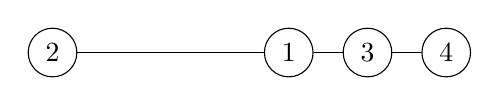
\begin{tikzpicture}
\node [draw, circle] (a) at (0,0) {1};
\node [draw, circle] (b) at (-3,0) {2};
\node [draw, circle] (c) at (1,0) {3};
\node [draw, circle] (d) at (2,0) {4};
\path [-] (a) edge node[left] {} (b);
\path [-] (a) edge node[left] {} (c);
\path [-] (c) edge node[left] {} (d);
\end{tikzpicture}
%\caption{$2$-Torus $T^2 = S^1\times S^1$. }
\end{center}
\end{figure}
\end{itemize}
\end{frame}

\section{The Algorithm}

\subsection{Description}

\begin{frame}{The Algorithm}
Let $x_1, \cdots, x_k\in\mathbb{R}^N$.
\begin{enumerate}
\item \textbf{Construct a weighted graph} $G=(V, E)$ with $k$ nodes, one for each point, and a set of edges connecting neighbouring points.
\textbf{Select a distance function}:
\begin{itemize}
\item (Euclidean Distance) Let $\varepsilon>0$. We connect and edge between $i$ and $j$ if $||x_i-x_j||^2 < \varepsilon$.
\item $n$ nearest neighbours. 
\end{itemize}
\pause
\item \textbf{Choose Weights}. If nodes $i$ and $j$ are connected, put
\begin{itemize}
\item $W_{ij}=1$.
\item (Heat Kernel) $W_{ij}\coloneqq e^{-\frac{||x_i-x_j||^2}{t}}$ for some $t > 0$.
\end{itemize} 
\pause
\item Assume $G$ is connected. \textbf{Compute the eigenvalues} of the generalized eigenvector problem $Lf = \lambda D f$, where
\begin{itemize}
\item $D$ is the diagonal weight matrix, $D_{ii} = \sum_{j=1}^k W_{ij}$.
\item $L\coloneqq D - W$ is the graph Laplacian. 
\end{itemize}
\pause
\item \textbf{Construct Embedding}. Let $f_0, f_1, \cdots, f_{k-1}$ be the corresponding eigenvectors ordered according to their eigenvalues ($\lambda_0 =0$). For $m<N$, set 
\begin{align*}
F(i)\coloneqq (f_1(i), \cdots, f_{m}(i)).
\end{align*} 
\end{enumerate}
\end{frame}


\subsection{Justification}

\begin{frame}{Why does it work?}{$m=1$}
Assume you have constructed the weighted graph $G=(V, E)$. We want to construct an embedding $F: V\longrightarrow\mathbb{R}$.\\
\vspace{0.3cm}
\underline{Hint:} Minimize
\begin{align*}
J(y)\coloneqq \sum_{i,j=1}^k (y_i - y_j)^2 W_{ij} \stackrel{*}{=} 2 y^\dagger L y.
\end{align*}
\pause
Thus, the problem reduces to find
\begin{align*}
\argmin_{\substack{
y^\dagger D y = 1\\
y^\dagger D 1 = 0}}
y^\dagger L y
=
\argmin_{\substack{
y^\dagger D y = 1\\
y^\dagger D 1 = 0}}
\langle Ly, y \rangle 
\end{align*}
\begin{itemize}
\item $y^\dagger D y = 1$ fixes the scale. 
\item $y^\dagger D 1 = 0$ eliminates the trivial solution $y=1$.
\end{itemize}
\pause
This translates to finding the minimum non-zero eigenvalue and eigenvector of 
\begin{align*}
Ly=\lambda D y.
\end{align*} 
\end{frame}

\begin{frame}{Why does it work?}{$m>1$ (Vectorize)}
Assume you have constructed the weighted graph $G=(V, E)$. We want to construct an embedding $F: V\longrightarrow\mathbb{R}^m$.\\
\vspace{0.3cm}
\underline{Hint:} Minimize, for $Y=(y_1 \cdots y_m)\in M_{k\times m}(\mathbb{R})$, 
\begin{align*}
J(Y)\coloneqq \sum_{i,j=1}^k ||Y_i - Y_j||^2 W_{ij} = \text{tr}(Y^\dagger L Y).
\end{align*}
Thus, the problem reduces to find
\begin{align*}
\argmin_{\substack{
\text{tr}(Y^\dagger D Y = I)}}
\text{tr}(Y^\dagger L Y)
\end{align*}
This translates to finding the minimum non-zero eigenvalues and eigenvectors of 
\begin{align*}
Lf=\lambda D y.
\end{align*} 
\end{frame}

\section{Examples: Scikit-Learn}


\begin{frame}{Examples: Scikit-Learn}

Let us go to a Jupyter notebook to see some examples.

\end{frame}

\section{Spectral Geometry*}

\subsection{The Laplacian}

\begin{frame}{The Laplacian}
Second order differential operator  
$L:C_c^\infty(M)\longrightarrow C_c^\infty(M)$.
\begin{itemize}
\item For $M = \mathbb{R}^n$,  
\begin{align*}
L = -\sum_{i=1}^n \frac{\partial^2}{\partial x_i^2}
\end{align*}
\item For $(M, g)$ Riemannian manifold, 
% - \frac{1}{\sqrt{|g|}}\sum_{i=1}^n \frac{\partial}{\partial x_i}\left(\sum_{j=1}^n \sqrt{|g|} g^{ij}\frac{\partial}{\partial x_j}\right)
\begin{align*}
L = - \sum_{i=1}^n\sum_{j=1}^n g^{ij}\frac{\partial^2}{\partial x_i \partial x_j} + \text{lower order terms}.
\end{align*}
\pause
\end{itemize}
\begin{block}{Spectral Theorem (\cite{R1997})}
L is symmetric with respect to the inner product in $C^\infty_c(M)$,
\begin{align*}
(f,g)_{L^2} = \int_M f(x)g(x)  dx.
\end{align*}
If $M$ is compact, there exists an orthonormal basis of $L^2(M)$ consisting of eigenvectors of $L$. Each eigenvalue is real.
\end{block}
\end{frame}

\begin{frame}{Embedding trough Eigenmaps}
Let $(M, g)$ be a compact Riemannian manifold and $f:M\longrightarrow \mathbb{R}$. 
\begin{itemize}
\item If $x, z\in M$ are close, then
\begin{align*}
|f(x)-f(z)| \leq \text{dist}_M(x,z) ||\nabla f||+o(\text{dist}_M(x,z)).
\end{align*}
\pause
\item We want a map that best preserves locality on average,
\begin{align}\label{Eqn:argmin_f}
\argmin_{||f||_{L^2(M)}=1}\int_M ||\nabla f||^2 dx.
\end{align}
\pause
\item By Stokes' Theorem
\begin{align*}
\int_M ||\nabla f||^2 dx = \int_M (Lf)f dx = (Lf,f)_{L^2}.
\end{align*}
\item \eqref{Eqn:argmin_f} must be an eigenvalue of the Laplacian. 
\end{itemize}
\end{frame}

\begin{frame}{The Graph Laplacian as a Differential Operator}
\begin{figure}[h]
\begin{center}
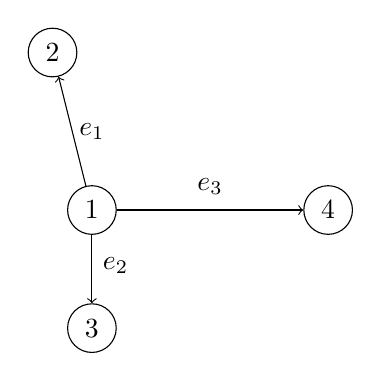
\begin{tikzpicture}
\node [draw, circle] (a) at (0,0) {1};
\node [draw, circle] (b) at (-0.5,2) {2};
\node [draw, circle] (c) at (0,-1.5) {3};
\node [draw, circle] (d) at (3,0) {4};
\path [->] (a) edge node[left] {} (c);
\path [<-] (b) edge node[left] {} (a);
\path [<-] (d) edge node[left] {} (a);
\node at (0, 1 ) {$e_1$};
\node at (0.3, -0.7 ) {$e_2$};
\node at (1.5, 0.3 ) {$e_3$};
\end{tikzpicture}
%\caption{$2$-Torus $T^2 = S^1\times S^1$. }
\end{center}
\end{figure}
\begin{align*}
\nabla = \left(
\begin{array}{cccc}
 -1 & 1 & 0 & 0 \\
 -1 & 0 & 1 & 0 \\
 -1 & 0 & 0 & 1
\end{array}
\right)
\quad 
\Rightarrow
\quad 
\nabla^\dagger \nabla = \left(
\begin{array}{cccc}
 3 & -1 & -1 & -1 \\
 -1 & 1 & 0 & 0 \\
 -1 & 0 & 1 & 0 \\
 -1 & 0 & 0 & 1 
\end{array}
\right)
\end{align*}
So we see, 
\begin{align*}
L = \nabla^\dagger \nabla. 
\end{align*}
\end{frame}

\subsection{The Heat Kernel}

\begin{frame}{The Heat Kernel}
Let $f:M\longrightarrow \mathbb{R}$. Consider the \textbf{Heat Equation} on $M$, 
\begin{align*}
\left({\partial_t} + L\right)u(x,t)  = 0
\quad \text{with intitial condition}
\quad
u(x,0) = f(x).
\end{align*}
\pause
\begin{itemize}
\item The solution is given by (\cite{R1997})
\begin{align*}
u(x,t) = \int_{M} H_t(x,y)f(y) dy, 
\end{align*}
where the \textbf{Heat Kernel} has the form
\begin{align*}
H_t(x,y) = (4\pi t)^{-\text{dim}(M)/2} e^{-\frac{\text{dist}_M(x,y)^2}{4t}} (\phi(x,y) + O(t)),
\end{align*}
for certain $\phi$ is a smooth function with $\phi(x,x) = 1$. 
\pause
\item It can be shown that, for $x_1, \cdots, x_k \in M$ and $t>0$ small,
\begin{align*}
Lf(x_i) \approx \frac{1}{t}\left(f(x_i) - 
\frac{
\sum_{0 < ||x_i - x_j||^2 <\varepsilon}
e^{-\frac{||x_i - x_j||^2}{4t}}f(x_j) 
}
{
\sum_{0 < ||x_i - x_j||^2 <\varepsilon}
e^{-\frac{||x_i - x_j||^2}{4t}}
}
\right)
\end{align*}
which justifies $W_{ij}=e^{-\frac{||x_i - x_j||^2}{4t}}$. 
\end{itemize}
\end{frame}

\begin{frame}{References}{Slides and notebook available at juanitorduz.github.io}
\bibliographystyle{alpha}
\bibliography{references} 
\end{frame}

\end{document}





























